\section{Conceptos generales de arreglos}
\subsection{Objetivo}
En esta unidad, se busca que el estudiante pueda entender y comparar
las distintas representaciones internas de arreglos, determinando para
cada una:
\begin{itemize}
\item facilidad de manejo
\item rapidez de acceso
\end{itemize}
    
\subsection{Definición}
\label{sec:definicion}

\begin{quote}
  Un arreglo es un sistema de elementos del mismo tipo, indizado por
  un sistema de coordenadas enteras, que permite acceder y alterar
  elementos individuales .
\end{quote}

En la programación, los arreglos son de uso extendido, tal que en la
mayoría de lenguajes de programación, los arreglos están incluidos
entre los tipos primitivos, como los enteros y caracteres.

Ejemplos del uso de arreglos:
\begin{alltt}
 int arreglo [5] ;  {\em // indizado 0..4}
 int  matriz [5][10] ;  {\em // indizado 0..4 * 0..9}
 arregloPascal:  array [11..20, 1..5] of  integer ;  {\em // de tamaño 10 * 5}
\end{alltt}

Acceso de los elementos:
\begin{verbatim}
arreglo[3] = 4 ,
matriz [4,9] = 5 ;
arregloPascal [12, 3] = 100 ;
\end{verbatim}

\subsection{Problema}
\label{sec:problema}
En los ejemplos anteriores, vemos que la notación para acceder los
elementos es relativamente simple.  Sin embargo, para el compilador no
es tan simple, ya que implica una serie de cálculos relativamente
complejos. Aunque no tengamos problemas para conceptualizar un arreglo
bidimensional (una matriz) o tridimensional (un cubo), estas
estructuras deben ser puestos en memoria, la cual es unidimensional.

La razón principal, se debe a que cuando se declara un arreglo, la
variable que representa dicho arreglo es en realidad una apuntador al
\textbf{primer} elemento del arreglo, como es el caso de las variables
\textit{arreglo}, \textit{matriz} y \textit{arregloPascal} en los
ejemplos anteriores, y cada una de las sentencias de acceso anteriores
implica un cálculo basado sólo en la dirección del primer elemento y
las dimensiones declaradas de cada arreglo.  Notación

Para las secciones siguientes, utilizaremos la siguiente notación
\begin{table}[H]
  \centering
  \begin{tabular}{lp{4cm}p{4cm}}
    \hline
    parejas límite & $n_1$..$m_1$ * $n_2$..$m_2$ * ... * $n_k$..$m_k$ donde $n_x \leq m_x$ &Conjunto de límites, para cada dimensión del arreglo\\
    \hline
    elemento del arreglo & A[i,j,k,..]& Notación para acceder un elemento del arreglo, dada por las coordenadas\\
    \hline
    dirección de un elemento &\&A[i,j,k,..]&Dirección de un elemento individual\\
    \hline
    función de localización &  Loc (A[i,j,k,..])& Fórmula que nos permite calcular la posición, dentro del arreglo, de un elemento indizado\\
    \hline
    dirección inicial& $\alpha$ = \&A[$n_1$,$n_2$,...,$n_k$]& Dirección del primer elemento.\\
    \hline
  \end{tabular}
\end{table}

\section{ Arreglos lexicográficos }
\subsection{Almacenamiento lexicográfico}
La primera representación que estudiaremos, que es la usual en los
lenguajes de programación, es la que cada arreglo se es puesto en una
sola región de memoria, de forma contigua, y se tiene que reservar la
memoria para todos los posibles elementos del arreglo, aunque no se
estén utilizando.  De ahí el nombre de arreglos estáticos.

Como programadores, es fácil para nosotros abstraer estructras como
matrices y cubos de forma simple, con las siguientes instrucciones:

int matriz[4,5] ;

\begin{figure}[H]
  \centering
  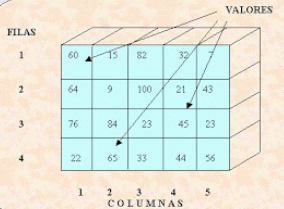
\includegraphics[scale=0.5]{2bidimensional}
\end{figure}

int cubo[2,2,8]
\begin{figure}[H]
  \centering
  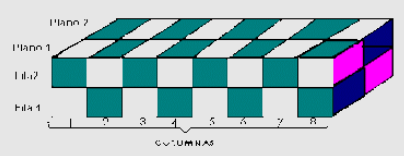
\includegraphics[scale=0.5]{2tridimensional}
\end{figure}

Estas estructuras las podemos trabajar con instrucciones como:

\begin{verbatim}
matriz[3,2] = 0 ;
o
int x = cubo [1,2,4] * 3 ;
\end{verbatim}

Sin embargo, debemos tomar en cuenta que, aunque el lenguaje nos
permita realizar este acceso fácilmente, la memoria de la computadora
no es multidimensional, y las matrices, cubos y arreglos de más de 3
dimensiones, deben poder mapear cada uno de los elemento, con una
coordenada única (conjunto de índices).

Esto implica que cada elemento debe tener un orden definido, de forma
que sea posible accederlo de forma inequívoca.  Dicho orden es el
orden lexicográfico:

\begin{definicion}
  \textbf{Orden lexicográfico por fila}: la posición ($a_1$, $a_2$
  ,..., $a_k$) es menor que ($b_1$, $b_2$,..., $b_k$), si y sólo si
  para algún $1 < j \leq k$, existe un $i$ tal que $a_i$ = $b_i$, para
  $1 \leq i < j$, y $a_j$ < $b_j$
\end{definicion}

Por ejemplo: si tenemos las coordenadas A=(1, 5, 1, 9) y B = (1, 5, 2,
8), el orden lexicográfico nos dice que A< B. En este caso k = 4,
entonces necesitamos un número entre 1 y 4 (la variable j), que sea el
índice de la coordenada tal que las coordenadas anteriores sean
iguales en A y B, y $a_j$ sea menor a $b_j$. En este caso, ese número
j corresponde a 3. Nótese que en la primera y segunda coordenada
tienen el mismo valor, y en la tercera se cumple que 1<2.

Dado que tenemos las dimensiones de una arreglo, y su dirección
inicial, es factible calcular la posición de cualquier elemento, dada
sus coordenada.  Lo cual veremos del caso más simple al caso general.

\subsection{Caso unidimensional}
\label{sec:caso-unidimensional}

Supongamos el siguiente vector $V$ de 4 elementos\\

\hspace{1in} $V: 1 .. 4$

\begin{center}
  \begin{tabular}{|c|c|c|c|}
    \hline
    1 & 2 & 3 & 4\\ \hline
  \end{tabular}
\end{center}

¿cuál sería la fórmula que nos permita mapear cualquier elemento de
este vector?  $Loc \left(V[i] \right)$ = ?

Por ejemplo: encontrar el elemento $V[3]$. Aquí, la dirección del
primero elemento es

$$ \alpha = \&V[1]$$

y

$$Loc \left( V[3] \right) =  \alpha + 2$$

Para encontrar el elemento $V[i]$

$$Loc \left( V[i] \right) = \alpha + i - 1$$

Si cambiamos la definición de $V$ a\\

\hspace{1in} $V:\; 10..13$

\begin{center}
  \begin{tabular}{|c|c|c|c|}
    \hline
    10 & 11 & 12 & 13\\ \hline
  \end{tabular}
\end{center}

aquí, la dirección del primero elemento es

$$ \alpha = \&V[10]$$

Entonces, para encontrar el elemento $V[12]$, ya no nos funcionaría la
fórmula anterior, dado que el índice inicial cambia de 1 a 10, por lo
tanto tenemos que cambiar a:

$$Loc \left( V[12] \right) = \alpha + 12 - 10$$

En general si tenemos un vector $V$ con pares límites arbitrarios así:

$$V: n_1..m_1$$

aquí, la dirección del primero elemento es

$$ \alpha = \&V[n_1]$$

Entonces, la fórmula cambia así:

$$ Loc \left( V[i] \right) =  \alpha + i - n_1$$

\subsection{Caso bidimensional}
\label{sec:caso-bidimensional}

Para el caso de una matriz (arreglo bidimensional), de 3*4 definida
como:

$$M:\; 1..3 * 1..4$$

aquí, la dirección del primero elemento es

$ \alpha = \&M[1,1]$

La conceptualizamos así:

\begin{center}
  \begin{tabular}{|c|c|c|c|}
    \hline
    1,1 & 1,2 & 1,3 & 1,4\\ \hline
    2,1 & 2,2 &	\textbf{2,3} & 2,4\\ \hline
    3,1 & 3,2 &	3,3 & 3,4\\ \hline
  \end{tabular}
\end{center}

Pero en memoria, realmente queda así:
\begin{center}
  \begin{tabular}{|c|c|c|c|c|c|c|c|c|c|c|c|}
    \hline
    1,1&1,2&1,3&1,4&2,1&2,2&\textbf{2,3}&2,4&3,1&3,2&3,3&3,4\\ \hline
  \end{tabular}
\end{center}

¿cuál sería la fórmula que nos permita mapear cualquier elemento de
esta matriz?  Si queremos encontrar el elemento M[2,3].

$$Loc \left( M[2,3]  \right) = \alpha + ?$$

Dado que el elemento está en la fila 2, sabemos que se debe avanzar
totalmente la primera fila (avanzarAFila), y luego aplicamos al
fórmula del vector, ya que cada fila es un vector.  Así:

$$Loc \left( M[2,3] \right) = \alpha + avanzarAFila(2) + 3 - 1$$

De esta forma tenemos que avanzar 4 elementos, ya que cada fila es de
tamaño 4.

$$ Loc \left( M[2,3] \right) = \alpha + 1 * 4 + 3 - 1 $$

Generalizando un poco más, si en esta matriz queremos encontrar un
elemento arbitriario $A[i,j]$ , aplicamos la fórmula así:

$$ Loc \left( M[2,3] \right) = \alpha + avanzarAFila(i) +  (j - 1) $$

Es decir debemos avanzar las filas necesarias para llegar a la fila $i$
y luego dentro de esa fila aplicamos la fórmula para un vector.

En general \textbf{\em avanzarAFila(i)}, se compone de dos elemento:
$FilasAntesDe(i) * TamanoDeCadaFila$, que en este caso son

\begin{eqnarray*}
  Loc \left( M[2,3] \right) &=& \alpha + FilasAntesDe(i)*TamanoDeCadaFila +  (j - 1)\\
  &=& \alpha + (i-1)*(4) +  (j - 1) 
\end{eqnarray*}

En general, si $M$ tiene pares límites arbitrarios, definida así:
$$M:\; n_1..m_1*n_2..m_2$$

aquí, la dirección del primero elemento es
$$\alpha = \&M[n_1,n_2]$$

y la fórmula cambia a:
\begin{eqnarray*}
Loc \left( A[i_1,i_2] \right) &=& \alpha + avanzarAFila(i_1) +  (i_2 - n_2)\\
&=&\alpha + FilasAntesDe(i_1)*TamanoDeCadaFila +  (i_2 - n_2)
\end{eqnarray*}

Dado que el límite inferior de la primera dimensión es $n_1$ entonces
$$FilasAntesDe(i_1) = i_1 - n_1$$

y, el tamaño de cada fila está dado por los límites de las columnas,
entonces
$$TamanoDeCadaFila = m_2 - n_2  + 1$$

Por lo tanto, la fórmula queda
$$Loc \left( A[i_1,i_2] \right) = \alpha + (i_1 - n_1)*(m_2 - n_2  + 1)  +  (i_2 - n_2)$$

\subsection{Caso tridimensional}
\label{sec:caso-tridimensional}
Sea el cubo

$$ C:\; 1..3 * 1..4 * 1..2 $$

aquí, la dirección del primer elemento es

$$ \alpha = \&C[1,1,1]$$

Tener en cuenta que en este caso, tenemos que cada índice en la
primera dimensión representa una matriz y cada índice en la segunda
dimensión, representa una fila de la matriz correspondiente, y la
última dimensión representa un elemento individual.

Así, se se desea acceder el elemento A[2,3,2], aplicamos la siguiente
deducción

\begin{eqnarray*}
  Loc \left( C[2,3,2] \right) &=& \alpha + avanzarAMatriz(2) + AvanzarAFila(3) +  (2 - 1)\\
  &=& \alpha + MatricesAntesDe(2)*TamanoDeCadaMatriz \\
  & & + FilasAntesDe(3)*TamanoDeCadaFila + (1)
\end{eqnarray*}

Sabemos que

$$ TamanoDeCadaMatriz = Filas * Columnas = 4 * 2 = 8 $$

y

$$ MatricesAntesDe(2) = 1 $$

y

$$TamanoDeCadaFila=2$$

y

$$ FilasAntesDe(3) = 2 $$

Por lo tanto

$$Loc \left( C[2,3,2] \right) = \alpha + (1)*8 + (2)*2 + (1) = \alpha + 13$$

En general, si C tiene pares límites arbitrarios,  así:

$$C: n_1..m_1 * n_2..m_2 * n_3..m_3$$

aquí, la dirección del primero elemento es

$$ \alpha = \&C[n_1, n_2, n_3]$$

y la fórmula cambia a:
\begin{eqnarray*}
  Loc \left( C[i_1, i_2, i_3] \right) &=& \alpha + avanzarAMatriz(i_1) + AvanzarAFila(i_2) \\
  & & + AvanzarAlElemento(i_3)\\
  \\
  &=& \alpha+\textcolor{red}{MatricesAntesDe(i_1)}*\textcolor{blue}{TamanoDeCadaMatriz}\\
  & &+\textcolor{cyan}{FilasAntesDe(i_2)} * \textcolor{green}{TamanoDeCadaFila}+(i_3-n_3)\\
  \\
  &=& \alpha + \textcolor{red}{(i_1-n_1)}* \textcolor{blue}{(m_2-n_2+1)*(m_3-n_3+1)}\\
  & &+\textcolor{cyan}{(i_2-n_2)}*\textcolor{green}{(m_3-n_3+1)}+(i_3-n_3)
\end{eqnarray*}

\subsection{Caso k-dimensional}
\label{sec:caso-k-dimensional}

Sea el siguiente arreglo k-dimensional

$$A:\;n_1..m_1 * n_2..m_2 * ... * n_k..m_k$$

aquí, la dirección del primero elemento es

$$ \alpha = \&A[n_1, n2,..., n_k]$$

Entonces deducimos la fórmula así:

\begin{eqnarray*}
  Loc \left( A[i_1, i_2, ... ,i_k] \right) &=& \alpha + ElementosDimension_1AntesDe(i_1)\\
  & & + ElementosDimension_2AntesDe( i_2)+ .... \\
  & & + ElementosDimension_{k-1}AntesDe (i_{k-1}) \\
  & & + AvanzarAlElemento(i_k)
\end{eqnarray*}

Sabemos que
$$ElementosDimension_xAntesDe(i_x) = (i_x -  n_x) * TamanoDeCadaElementoEnDimension_x$$

y para calcular el $TamanoDeCadaElementoEnDimension_x$ , revisemos los
casos anteriores:

\begin{description}
\item[Tamaño de cada elemento en la última dimensión: ]
  $$1$$
\item[Tamaño de la ultima fila (dimensión k-1): ]
  $$ m_k - n_k + 1$$
\item[Tamaño de la última matriz ( dimension k -2 ): ]
  $$(m_{k-1} - n_{k-1} + 1) * (m_k - n_k + 1) $$
\item[Tamaño del último cubo (dimensión k-3): ]
  $$(m_{k-2} - n_{k-2} + 1) * (m_{k-1} - n_{k-1} + 1) * (m_k - n_k + 1) $$
\item[...]
\item[Tamaño de la dimensión k-j: ]
  $$(m_{k-j+1} - n_{k-j+1} +1) * ...* (m_{k-1} - n_{k-1} + 1) * (m_k - n_k + 1) $$
\item[...]
\item[Tamaño de la primera dimensión (cuando k-j=1 y k-j+1=2): ]
  $$(m_2 - n_2 +1) * ...* (m_{k-1} - n_{k-1} + 1) * (m_k - n_k + 1)$$
\end{description}

Por lo tanto:
\begin{eqnarray*}
  Loc (A[i_1, i_2, ... ,i_k]) &=& \alpha + (i_1 - n_1) *(m_2 - n_2 -1) * ...* (m_{k-1} - n_{k-1} + 1) * (m_k - n_k + 1)\\
  & & + (i_2 - n_2) *(m_3 - n_3 -1) * ...* (m_{k-1} - n_{k-1} + 1) * (m_k - n_k + 1)\\
  & & + (i_3 - n_3) *(m_4 - n_4 -1) * ...* (m_{k-1} - n_{k-1} + 1) * (m_k - n_k + 1)\\
  & & +.........+\\
  & & + (i_{k-1} - n_{k-1}) * (m_k - n_k + 1)\\
  & & + (i_k - n_k) 
\end{eqnarray*}

\[
Loc (A[i_1, i_2, ... ,i_k])= \alpha + \sum_{x=1}^k \left[(i_x-n_x) \prod_{y=x+1}^k\left(m_y-n_y+1\right)\right]
\]

\subsubsection{Ejemplo}
\label{sec:ejemplo}

\begin{definicion}
  \textbf{Orden lexicográfico por columna}. La posición $(a_1, a_2 ,
  \ldots , a_k)$ es menor que $(b_1, b_2, \ldots , b_k)$, si y sólo si
  para algún $1 < j \leq k$, existe un $i$ tal que $a_i = b_i$, para
  todo $j < i \leq k$, y $a_j < b_j$
\end{definicion}

$$\text{Ej.} Matriz:\; 1..3 * 1..4$$
\begin{center}
  \begin{tabular}{|c|c|c|c|}
    \hline
    1,1 & 1,2 & 1,3 & 1,4\\ \hline
    2,1 & 2,2 &	\textbf{2,3} & 2,4\\ \hline
    3,1 & 3,2 &	3,3 & 3,4\\ \hline
  \end{tabular}
\end{center}

Se almacena así:
\begin{center}
  \begin{tabular}{|c|c|c|c|c|c|c|c|c|c|c|c|}
    \hline
    1,1&1,2&1,3&1,4&2,1&2,2&\textbf{2,3}&2,4&3,1&3,2&3,3&3,4\\ \hline
  \end{tabular}
\end{center}

sea $A$ un arreglo de $n_1..m_1 * n_2..m_2$ ordenado
lexicográficamente por columnas. Deducir $LOC \left( A[i,j] \right) =
\alpha + (j-n_2) * (m_1-n_1+1) + (i-n_1)$

En general, para el arreglo $A:\; n_1..m_1 * n_2..m_2 * .... * n_k..m_k$

\begin{eqnarray*}
  LOC \left( A[i_1, i_2, .., ik] \right) &=& \alpha + (i_k - n_k)* (m_1 - n_1 +1) * (m_2 - n_2 + 1) * ...* (m_{k-1} - n_{k-1}  +1 )\\
  & & + (i_{k-1} - n_{k-1} ) * (m_1 - n_1 +1) * (m_2 - n_2 + 1) * ...* (m_{k-2} - n_{k-2}  +1 ) + \\
  & &  \ldots \\
  & &  (i_2 - n_2 ) * (m_1 - n_1 +1)  + \\
  & & (i_1 - n_1 )
\end{eqnarray*}




\section{Arreglos esparcidos}
Vimos que el uso de arreglos lexicográficos tiene el mejor rendimiento
posible (constante) para el acceso de elementos por índice.  Sin
embargo, el hecho de que necesiten reservar memoria contigua para
todos sus posibles elementos, implica que existen situaciones en las
que no son recomendables, debido principalmente a dos factores:

\begin{enumerate}
\item Desperdicio de memoria: consideremos una matriz de 1,000 por 1,000
elementos, de los cuales sólo se están utilizado 10. Sería un gran
desperdicio de memoria, alojar 1,000,000 de elementos para sólo
utilizar 10.
\item Incapacidad de alojar espacio para todos los posibles elementos: las
hojas electrónicas tienen una gran capacidad de celdas, pero
normalmente sólo se utiliza una pequeña porción de ellas: Excel tiene
su máxima celda en IV65536, lo que significa una capacidad para
(26*8+22)*65536 = 15,073,280 celdas.  Si cada una de estas ocupara 1
byte, no tendríamos memoria suficiente para una hoja electrónica..
\end{enumerate}


En cualquiera de estos casos resultan útiles los arreglos esparcidos,
los cuales tienen como característica fundamental que \textbf{sólo utilizan la
memoria realmente necesaria conforme se agregan elementos al arreglo}.

\subsection{Técnicas de representación}

Entre muchas técnicas para lograr los arreglos esparcidos,
distinguiremos dos principales:
\begin{itemize}
\item Arreglos lexicográficos de encabezados, con celdas de referencias cruzadas.
\item Listas de encablezados
\end{itemize}

El uso de arreglos lexicográficos para los encabezados se ilustran en
la siguiente figura:
\begin{figure}[H]
  \centering
  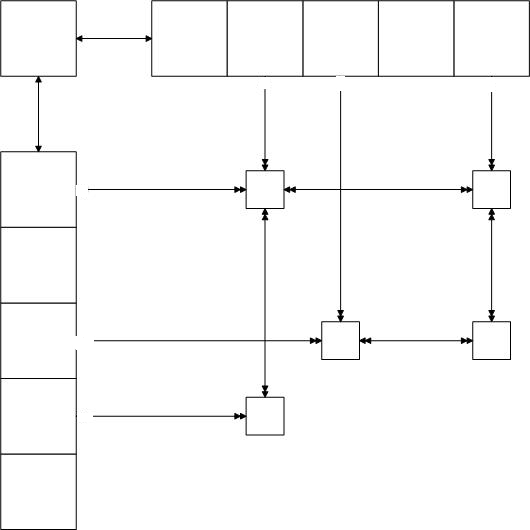
\includegraphics[scale=0.6]{3arregloLexografico}
\end{figure}

Se tiene un control de encabezados, el cual contiene dos apuntadores:
uno para el arreglo de las filas y el otro para las columnas.  Los
encabezados no necesitan más información que el apuntador al primer
nodo de la fila o columna.  Cada uno de los nodos tiene la siguiente
estructura:
\begin{figure}[H]
  \centering
  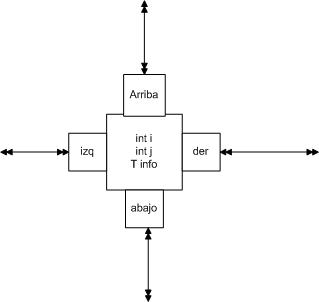
\includegraphics[scale=0.7]{3nodo.jpeg}
\end{figure}

Los cuatro apuntadores de navegación nos sirven para facilitar los
recorridos y búsqueda de cada nodo.  Notemos que, además de la info,
se debe tener en cada nodo la información de los índices que
representan, ya que la caraterística de esparcido no permite calcular
el índice de un nodo basado en sus posición de forma fácil.  Se podría
omitir esta información, para para buscar cada nodo implicaría una
doble búsqueda, por fila y columna, para cada nodo, lo cual lo haría
muy ineficiente.

La estrategia básica del algoritmo de localización de un elemento
A[i,j]

\begin{alltt}
   {\it Seleccionar el encabezado de las filas, aunque también puede ser por columna
   Para cada nodo en la lista de la fila {\bf i}}
  
   Si {\bf nodo.j < j}
        nodo = nodo.der  ; {\it //seguimos buscando}
   sino
        si {\bf nodo.j=j}
             return {\bf nodo} ; {\it // encontramos el nodo}
        {\bf sino}
             return null ;  {\it // no se encuentra el nodo con los índices indicados}
        fin
   fin 
\end{alltt}

Una implementación más formal, podría ser la siguiente:

\begin{verbatim}
public class ArregloEsparcido<E> extends ArregloGeneral<E> {
.
.
.
       public  E get (int i[]) {
            /* resumiendo a búsqueda por filas */
            Nodo n = fila [i] ;

            while (n != null &&  n.col < j) {
                n = n.derecha ;
            }
            if ( n == null )
                return null ;
            else
                return n.obj ;
       }
.
.
.
}
\end{verbatim}

Analizando el orden de este algoritmo:
\begin{itemize}
\item El peor de los casos es una matriz de una solo fila, la cual está
llena y estamos buscando el último elemento de dicha fila.  En este
caso el O(get(i)) = n, es decir lineal, ya que visitaremos todos los
elementos.
\item Si fuera una matriz cuadrada totalmente llena, entonces n = filas *
columnas y filas = columnas = x , por lo tanto $n = x^2$ .  Al hacer la
búsqueda del último elemento de cada fila, recorreremos x elementos,
es decir O(get(i)) = sqrt(n).
\item En el caso general, en que las filas != columnas, O(get(i)) =
  n/columnas, es decir se convierte en sublineal.
\end{itemize}

Por lo tanto el orden de este algoritmo varia de lineal a sublineal,
dependiendo de la estructura de la matriz.

Las otra técnica de representación está basada en que también los
encabezados son listas, en vez de arreglos lexicográficos.  Así, otra
representación de la matriz anterior es así:
\begin{figure}[H]
  \centering
  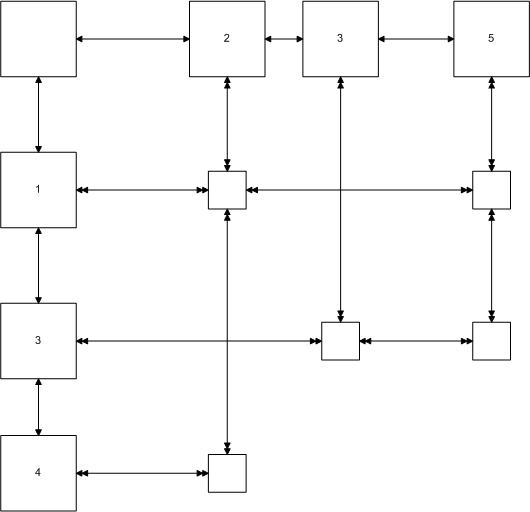
\includegraphics[scale=0.5]{3encabezadosLista.jpeg}
\end{figure}

Aquí los nodos de los encabezados tendrían la siguiente estructura:
\begin{figure}[H]
  \centering
  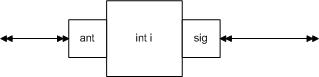
\includegraphics[scale=0.8]{3nodoEncabezadoLista.jpeg}
\end{figure}

Esta representación al seguir manteniendo los nodos con doble enlace
en ambas dimensiones, permite tener la misma flexibilidad en el
recorrido de elementos que la representación con encabezados de
arreglos.  La diferencia básica es que el recorrido en los
encabezados.  Sin embargo, cuando se tienen múltiples dimensiones,
mantener en los nodos el doble enlace hacia cualquier dirección,
complica de gran manera las operaciones de inserción y eliminación,
además de representar un consumo alto de memoria por uso de dos
apuntadores por nodo, por dimensión.  Para estos casos se podría
utilizar una representación como la siguiente:

\begin{center}
  arreglos-ortogonales-listas2
\end{center}

En este caso, los nodos de información ya no necesitan almacenar ni
apuntadores, ni índices de la posición que representa, ya que dicha
posición, es determinada en el recorrido de los encabezados.

El almacenamiento encadenado puede ser útil para acomodar el
crecimientos de los arreglos en direcciones arbitrarias, a costa de de
una utilización de espacio reducido

\subsection{Comparación de técnicas}
\label{sec:comp-de-tecn}

El rendimiento del acceso a los arreglos, está dado por la
representación interna

\subsubsection{Criterios de comparación}
\label{sec:crit-de-comp}

\begin{itemize}
\item simplicidad de acceso a los elementos
\item facilidad de recorridos en diferentes rutas
\item eficiencia de uso del almacenamiento
\item facilidad de crecimiento
\end{itemize}

\subsubsection{Almacenamiento lexicográfico vs esparcido}
\label{sec:almac-lexic-vs}

\paragraph{Ventajas}
\label{sec:ventajas}

\begin{itemize}
\item cálculo fácil ( O(n) = c )
\item facilidad de recorrido
\item crecimiento fácil en la primera dimensión
\end{itemize}

\paragraph{Desventajas}
\label{sec:desventajas}

\begin{itemize}
\item crecimiento muy costos en las otras dimensiones
\item Uso de la memoria sólo es óptimo si está lleno (o casi lleno).
  Radio = ( tam(objeto) / tam(objeto + apuntadores) ) indica el máximo
  porcentaje de llenado a partir del cual es más eficiente un arreglo
  lexicográfico.
\end{itemize}



%%% Local Variables:
%%% TeX-master: "tedd"
%%% End:


% expresiones regulares, en su momento,  utiles para este doc:
% \([[:alpha:]]\)\([[:digit:]]\) -> \1_\2